\documentclass[conference]{IEEEtran}
\IEEEoverridecommandlockouts
% The preceding line is only needed to identify funding in the first footnote. If that is unneeded, please comment it out.
\usepackage{cite}
\usepackage{amsmath,amssymb,amsfonts}
\usepackage{algorithmic}
\usepackage{graphicx}
\usepackage{textcomp}
\usepackage{xcolor}


% hyperlinks

\usepackage{listings}
\usepackage{xcolor}

\definecolor{codegreen}{rgb}{0,0.6,0}
\definecolor{codegray}{rgb}{0.5,0.5,0.5}
\definecolor{codepurple}{rgb}{0.58,0,0.82}
\definecolor{backcolour}{rgb}{0.95,0.95,0.92}

\lstdefinestyle{mystyle}{
    backgroundcolor=\color{backcolour},   
    commentstyle=\color{codegreen},
    keywordstyle=\color{magenta},
    numberstyle=\tiny\color{codegray},
    stringstyle=\color{codepurple},
    basicstyle=\ttfamily\footnotesize,
    breakatwhitespace=false,
    breaklines=true,                 
    captionpos=b,                    
    keepspaces=true,                 
    numbers=left,                    
    numbersep=1pt,                  
    showspaces=false,                
    showstringspaces=false,
    showtabs=false,                  
    tabsize=2
}

\lstset{style=mystyle}

\def\BibTeX{{\rm B\kern-.05em{\sc i\kern-.025em b}\kern-.08em
    T\kern-.1667em\lower.7ex\hbox{E}\kern-.125emX}}
\begin{document}

\title{GeoMedia: A Platform to Share Comments and Multimedia Content Based on Location.\\
}

\author{\IEEEauthorblockN{ Alberto Morini}
\IEEEauthorblockA{\textit{Department of Mathematics} \\
\textit{University of Padua}\\
Padua, Italy \\
alberto.morini@studenti.unipd.it
}
\and
\IEEEauthorblockN{ Prof. Claudio Enrico Palazzi}
\IEEEauthorblockA{\textit{Department of Mathematics} \\
\textit{University of Padua}\\
Padua, Italy \\
cpalazzi@math.unipd.it}
}

\maketitle

\begin{abstract}
Nowadays Online Social Networks (OSN) are the principal way to create connections among people and discover places.
Platforms like Facebook, Twitter, and Instagram suggest content and profiles based not only on mutual connections or trending content but also on geographic location of the end-user.
\\
GeoMedia is a platform, developed as an Android mobile application, which provide a medium for users to share comments and multimedia content (such as photos, videos, and audio) based on their location.
Then, users can easily see the content shared through GeoMedia moving across a geographical map.
\end{abstract}

\begin{IEEEkeywords}
Android, Social Networks, geolocation, microservices, client server, multimedia, media sharing, android location, http, three-tier, three-tier architecture, SQL, DBMS
\end{IEEEkeywords}

\section{Introduction}
In the last decade, mobile applications have almost replaced traditional computer programs, especially when it comes to social networks. Not only because it is more convenient to use a mobile phone than a laptop, but also because mobile phones can give more functionality by using the physical sensors present in way to enrich the user experience.


The explosion of OSN led media companies to invest and explore almost all functionality of mobile devices, thus to make users feel more connected and satisfied by providing more relevant content. As a result, users spend more time on these platforms, generating profit for social media companies.
A perfect example is Tinder, a dating app where users can meet each other based on their geographical proximity.
To reach this purpose, a variety of sensors can be used to profile the end user, often using the GPS to get the precise location, otherwise opting to the proximal location provided by Access Point / Cell antenna.

However, utilizing these features can lead to faster battery drain, higher data usage, and potential privacy concerns.
GeoMedia represents an open-source alternative, which does not share data to third systems and access to only necessary user information; so limiting the energy consumption and protecting users' privacy.
\\

\section{Related works}

As slightly mentioned before, online social media are growing exponentially in terms of numbers and also of functionality provided; in fact, there are several alternatives to GeoMedia but more complex and more invasive in terms of privacy.
In example
\subsection{Google Maps}
Google Maps\cite{GoogleMaps} is a web mapping platform providing many functionality such as: route directions, traffic conditions and ``Street View"\cite{StreetView} which function consent users to create an immersive 360\textdegree vision in a specific point on the map.
The last function is the only way to enrich the geographical map with data, but on the other hand is very complex to create a content because it's not a picture or a video but a full panoramic.
Furthermore, it's not possible to insert a simple description text.
\\
Another functionality which allows users to write and post media content (limited to photos or videos) is a reviews or rating of a place such as a bar, museum or attraction point already created by the platform or the owner of the by the business.

\subsection{Foursquare City Guide}

Another Online Social Network that can be used to explore location or share comments across a city, was Foursquare City Guide\cite{FourSquareWiki} owned by Foursquare Labs Inc. \cite{FoursquareOfficialLink} created in 2008, that shut down in October 2024.
The app provides personalized recommendations of places near a user's current location based on users' previous browsing history and check-in history, allowing users to upload content in the position they are.
\\
After the shut down, the features of this social network will be earned by SwarmApp \cite{FoursquareSwarm}, another online social network owned by the same comapany, that allows users to send their location to their friends.


\subsection{Instagram}
Instagram \cite{Instagram} is one of the biggest Online Social Networks of the last decade in terms of active users; the platform is profile-centric by allowing users to enrich their profile with photos or video, and potentially to manually add a location to the post by selecting a nearly place or searching a position (i.e. a museum, a bar, a city).
\\
With this functionality, Instagram offers also the possibility to navigate through a map seeing various content published, but cannot limit posts to a defined geographical area.
The only exclusivity that Instagram can give is with the ``Instagram stories", a feature which limit photos or videos from the moment of publication up to the next 24 hours.
\\
Even Instagram can retrieve the location via GPS to place the position in the map near to the end users.

In the end, this platform has a backbone ready to makes what GeoMedia do but not properly centered on that. Another aspect that users might consider is relative to the privacy concerns, since the social network is owned by by Meta Platforms, Inc. a profit company which is well known to share personal data to third parts\cite{MetaPrivacy}



\section{GeoMedia}

GeoMedia insert itself among the others Online Social Networks (OSNS), offering another way to share content in order to discover new places by adding a comment or a multimedia file in the current user location.
In fact, the app provides just a geographical map, where users can fill it by posting photos, audios, videos, or just text. So, users are in charge of enriching the map of a city by creating a post, then for example, giving others the opportunity to discover secrets spots or facts about a place.
Unlike ohters app seen before (i.e. Google Maps), the mobile app automatically get the position of the user posting by retrieving the information from the GPS placed inside the phones, bringing the online social network into the physical world. In fact, the app provides the feature to create some exclusive content by choosing to restrict the post published just in a determinate date and time or in a well defined geographical area.

An interesting scenario could be adopted by the city of Pauda to explain one of it's dictum: ``città dei tre senza" (city without the three).
Which consists in three things that Padua has but not in a proper way:
\begin{itemize}
    \item \textit{The Lawn Without Grass}, which is ``Prato della Valle" because the grass in it, is just ornamental is not really really a lawn like the word would intend
    \item \textit{Saint without a name}, which is ``Saint Anthony of Padua" (Sant'Antonio da Padova) except that he wasn't from Padua, but from Portugal; and the friar only lived the last of his years in Padua
    \item \textit{Coffee without doors}, and this is the ``Pedrocchi Coffee", because during war time was open all day (so the doors was removed) to provide shelter during the bombings.
\end{itemize}
So, the city of Padua could use GeoMedia to place some comments in these locations to tell the story of each particularity or even upload old photos to show as it was.
\\

In the end, GeoMedia, offers a full solution to share contents in the location of where the end users is, making the Online Social Network (OSN) interactive with the real world and without the effort to pick the right location as usually happens with other social networks app

The whole source code developed for this project is available on GitHub. \cite{gh}


\section{Architecture}\label{Architecture:panoramic}

To ensure that the GeoMedia app functions as intended, it is necessary to design an opportune architecture, even if it is not strictly related to the mobile application itself.
In fact, the adopted three-tier architecture makes the app work as intended, as shown in Figure 1.
The architecture is composed of three actors: the presentation layer, the application layer, and the data layer.

\begin{figure}[htbp]
{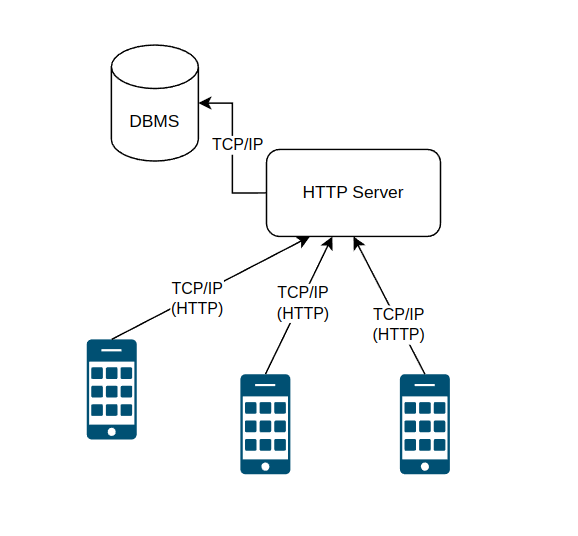
\includegraphics[width=9.5cm]{imgs/Architecture.png}}
\caption{Three-tier architecture for GeoMedia.}
\label{fig}
\end{figure}


\subsection{Presentation layer}
Presentation layer also called client layer, is represented by mobile phones since GeoMedia is the Android app that serves as an interaction point with users and the designed back-end architecture.
\\
By providing a user interface, users can view the published comments or share their own content; which in the last case, the mobile app, as presentation layer, has also the duty to retrieve data such as the user's location, username and other metadata even if not directly inserted by the user.
\subsection{Application layer}

In this project, the application layer is represented by an HTTP server, by handling the requests received with the opportune functions and logic; for example, compute the distance from the given location to the exclusive posts.
The HTTP server exposes the endpoints that the front-end (presentation layer) will fetch by making some HTTP request.
\\
Specifically, for each endpoint, the server will manipulate the contents uploaded with opportune SQL instruction through the Data Layer.

\subsection{Data layer}

The Data Layer consists into a Database Management System (DBMS), capable of performing CRUD operations (Create, Read, Update, Delete) on data stored in defined tables.
\\
For this project, the DBMS will also be used to create SQL stored procedures, offering a more flexible way to modify the select or insert of data queries in future extensions, without changing the code inside the server program.


\section{Mobile application}
In way to create a mobile application, there are several frameworks and technologies options. For this project has been selected the ``Ionic Framework" \cite{b1}, an open source toolkit for building cross-platform mobile, web, and desktop applications using web technologies such as HTML, CSS, and JavaScript.
One of the key advantages of the Ionic Framework is its ability to integrate web frameworks like ReactJS, that offers many functionality such as the updates of data changed in the user interface, or some special functions called ``hooks" triggered on particular events that make possible the customizations and the injection of personalized functions.
For example, the React' hook ``useEffect()" allows to call functions at the component startup or when a property change, giving to the developer the entry point to call some personalized functions; or instead the hook ``useState()" allows an automatic refresh of components rendered in the user interface at the change of the data inside it.


\subsection{Key functionality }

GeoMedia starts with a log-in component, where users can choose to create a new profile or to sign in whenever they already have an account.
\\
Once logged into the app, GeoMedia offers a bottom menu with two sections: 
\begin{itemize}
    \item \textit{Profile}, in this tab users can see their posts as list and open them; or change the server configuration parameters (i.e. IP Address or HTTP port)
    \item  \textit{Map}, this section is the heart of the app, by offering a navigation through a geographical map to look for the comments and posts uploaded by other users. Furthermore this tab provide also the access to the publish component that allows users to create a new post based on their coordinates.
\end{itemize}

\\
A single post is composed of some attributes:
\begin{itemize}
    \item Title
    \item Comment
    \item Multimedia content (which is optional)
    \item And others metadata automatically retrieved (longitude, latitude, username, date, ...)
\end{itemize}

\subsection{Map component}

As cited before, the heart of GeoMedia app is the ``Map" component, that utilizes Pigeon Map\cite{b8}, which is a React component that encapsulates and provides a geographical interactive map; this library also allows to put some ``markers" in specific location (longitude and latitude), which in the case of GeoMedia those points represent a content posted.

\\

There are different types of location indicator:
\begin{itemize}
\item Blue marker: the current user location (retrieved in real time by GPS)
\item Red marker: a post with just a comment text
\item Yellow marker: a post with a media attached
\item Green marker: an exclusive post, so a content visible only at date and time or in a well defined geographical area range (i.e. within 5 km)
\end{itemize}

Respecting the three-tier model explained in Section \ref{Architecture:panoramic}, the client mobile application when fetching the server in order to retrieve data, provides the current position of the user. Then, the server as application layer, filters only the relative posts stored in the data layer; then returns an HTTP packet including the uploaded comments and multimedia data related.
The specific methods to filtering the exclusive content will explained in the dedicated subsection\ref{server:screening}


\\
As follows a snippet of Map Component created
\begin{lstlisting}[language=Java, caption=Map component snippet]
//various imports ...
import { useContext, useEffect, useState } from "react";
const MyPMap = () => { //declare the Map component

    const [PostList, setPostList] = useState([]) //to store the list of posts
    const ctx = useContext(mycontext)  //use the React context to retrieve data of other components
    
    function getPosts() {
        if (ctx?.UserPosition != null) {
            doRequest("getPosts", { //do an HTTP request to server
                latitude: ctx?.UserPosition[0]
                , longitude: ctx?.UserPosition[1]
            }).then(res => {
                setPostList(res)
            })
        } 
        ...
    }
    
    useEffect(() => {
        getPosts(); //to call the post
    }, []); //at the startup of component
    return( //render the graphics
        <>
        <Map defaultCenter={ctx?.UserPosition} defaultZoom={11}>
            <ZoomControl />
            <Marker width={50} anchor={ctx?.UserPosition} color={"#154c79"} />
            {
                PostList?.map(s => (
                    <Marker width={50} anchor={[s.LATITUDE, s.LONGITUDE]} color={(s?.MEDIATYPE?.length > 0) ? '#d6c531' : '#f23c3c'}
                        onClick={() => {
                            setPostSelected(s) //store the post selected to open it in the opportuned component (viewPost)
                        }}
                    />
                ))
            }
        </Map>
        ...
        </>
    );
}
export default MyPMap;
\end{lstlisting}

The results rendered by the Map component can be seen in Figure 2, where in the left scenario two cities are included, useful case to cover wider area such rural landscapes; instead, in the right image, there's a more detailed scenario that enrich the center of a town by marking interesting attraction points with photos and comments.

\begin{figure}
\begin{minipage}{.2\textwidth}
    \subfloat{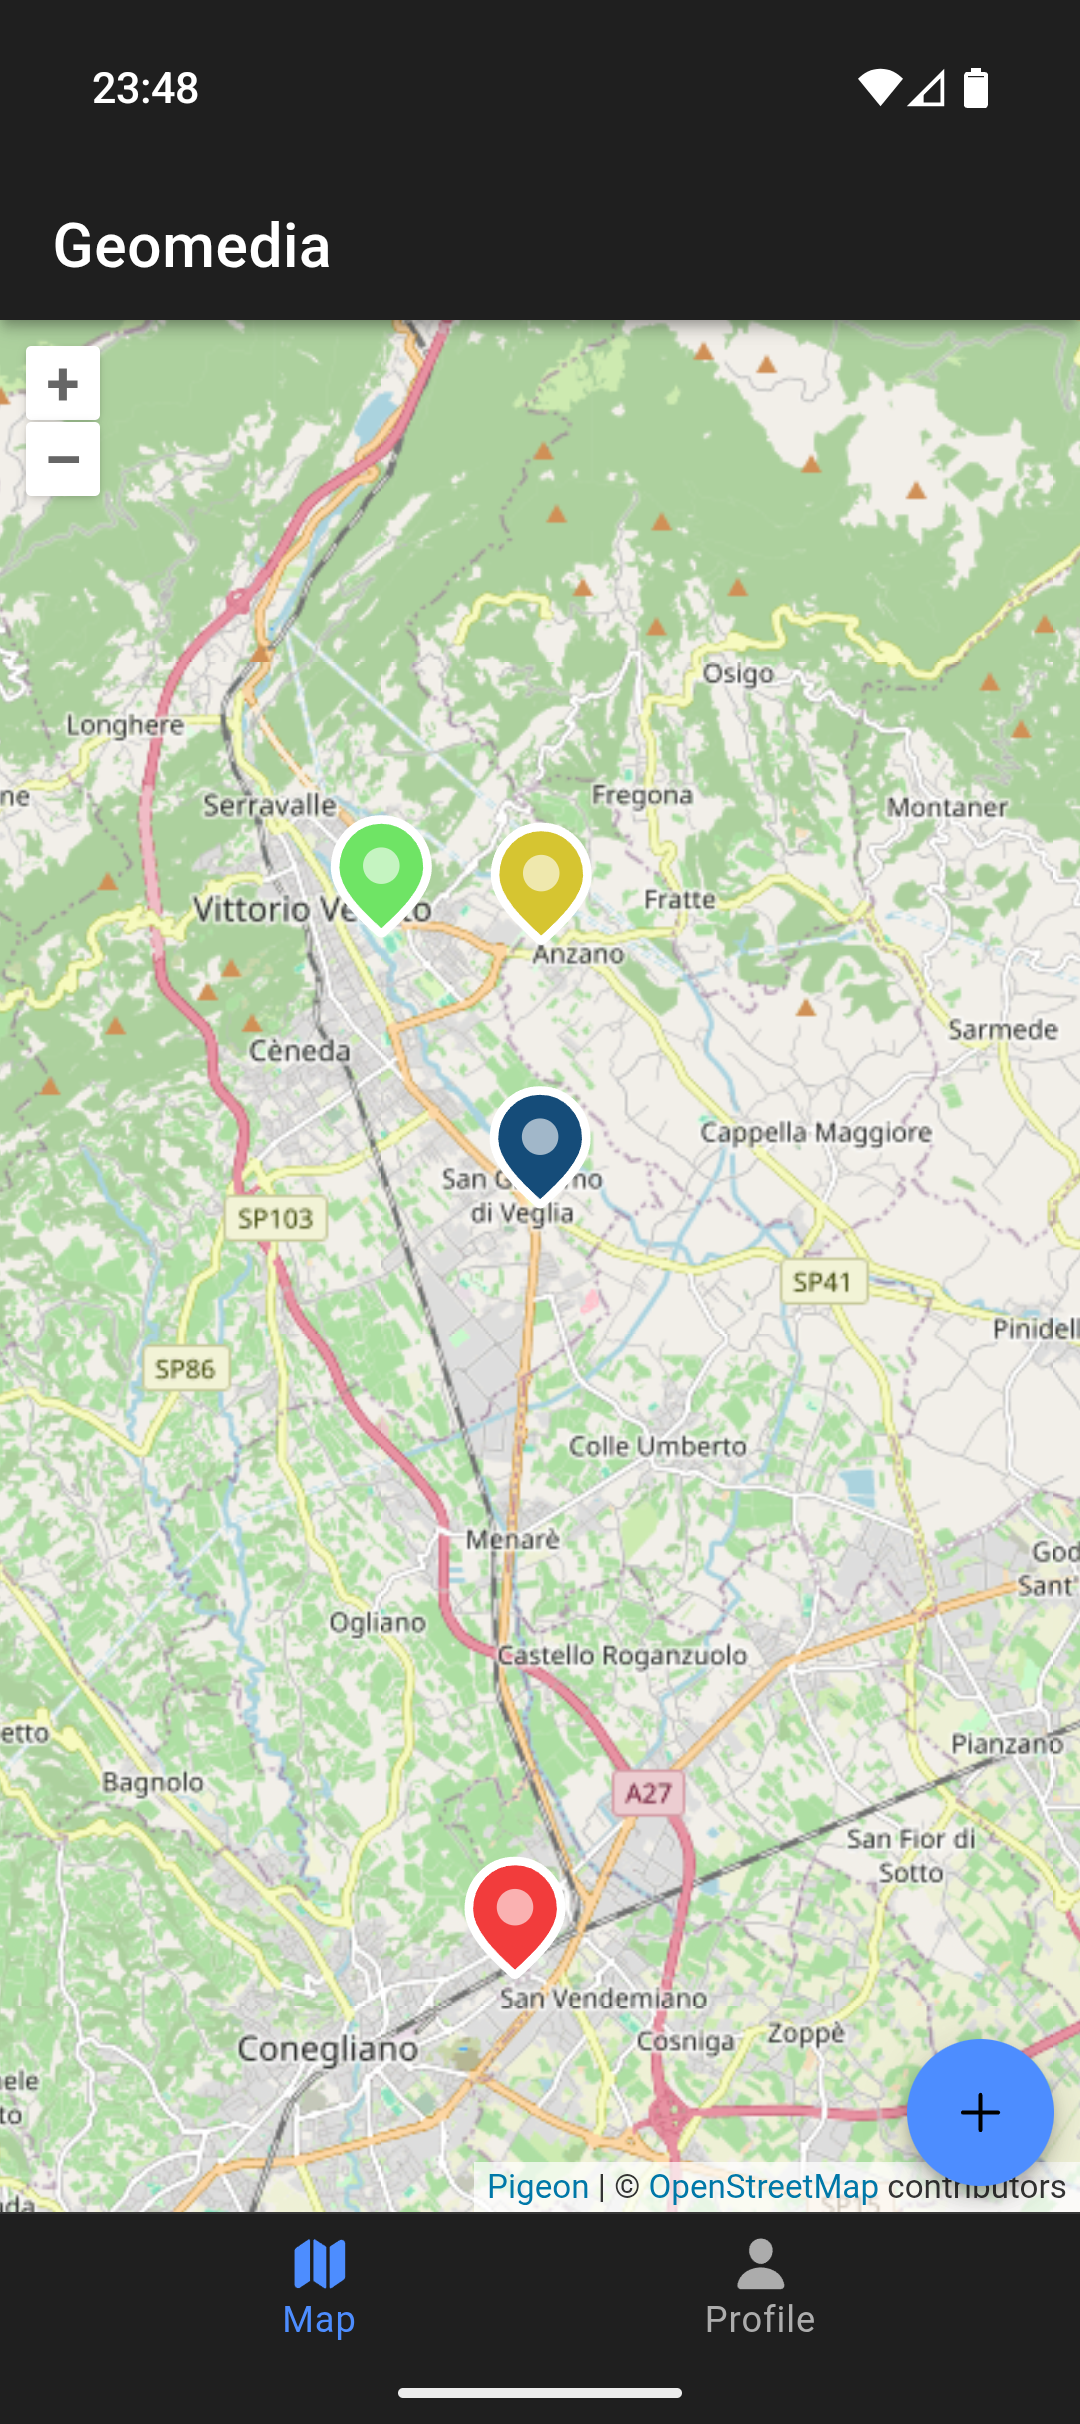
\includegraphics[width=\textwidth]{imgs/Screenshots/Panoramica.png}}\label{fig:sub_a}}
\end{minipage}
\hfill    
\begin{minipage}{.2\textwidth}
    \subfloat{\fbox{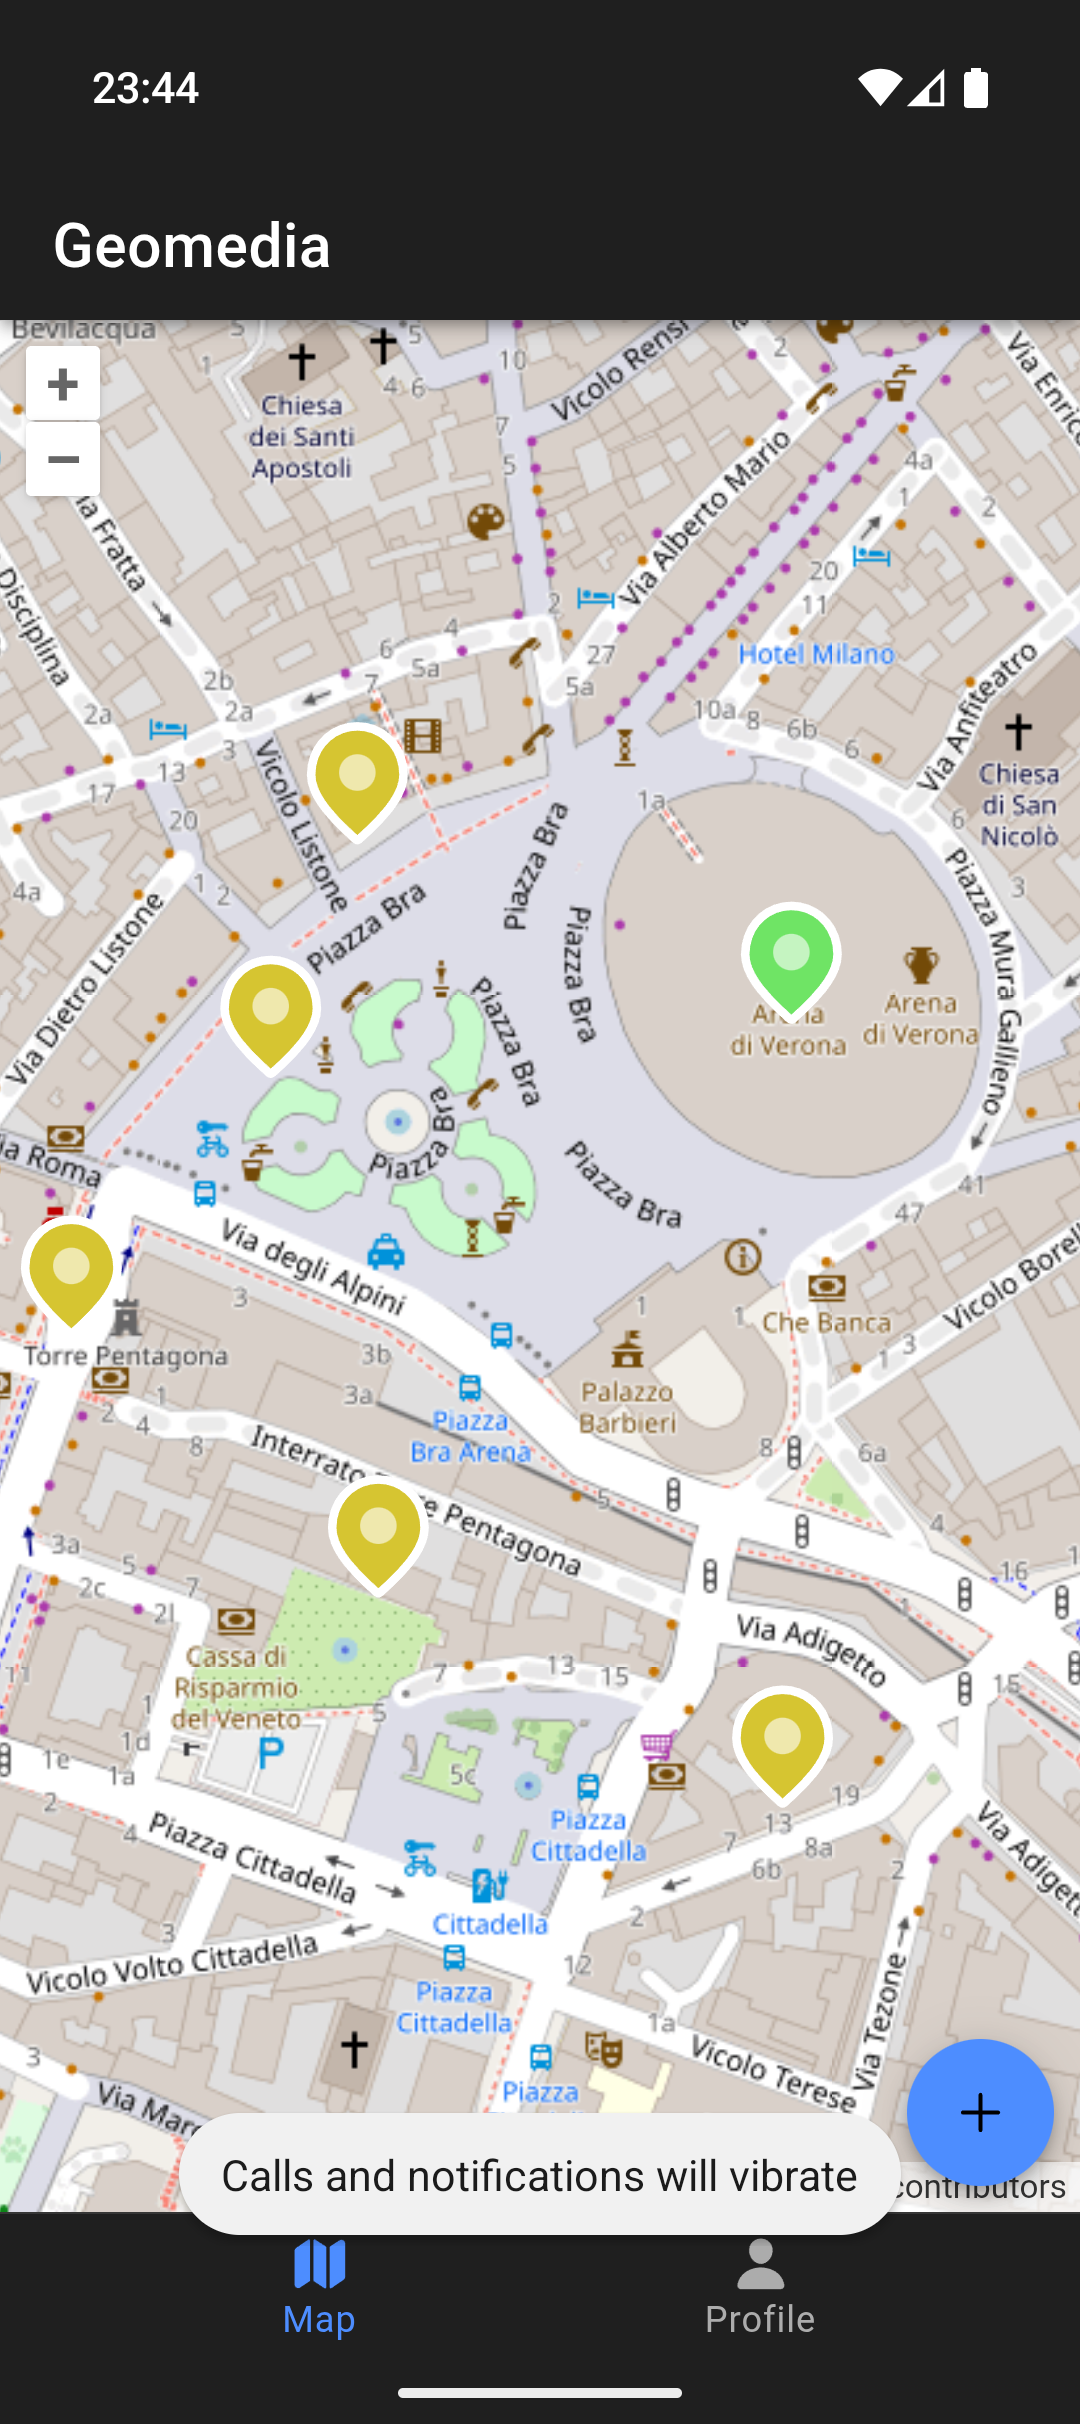
\includegraphics[width=\textwidth]{imgs/Screenshots/Centro.png}}}\label{fig:sub_b}}
\end{minipage}
    \caption{Example of rendered content by the Map component}\label{fig:sub}
\end{figure}


\subsection{Exclusivity}


GeoMedia makes users interact with the real world by retrieving the real location and then fetching the server to gets the contents around them.
In fact, a user, when creating a new post, can choose to make it exclusive by two factors: date or area.

An exclusive post by date will be visible from the moment it's been posted to the time indicated.
Moreover, users can choose a maximum distance within the content will be visible by others, so creating an area like a circle with at the center the location of user posting.

As explained before, limited content are represented by green markers, in fact, Figure 3 compared to the right Figure 2, proves the correctly of GeoMedia by retrieving a post limited by area when the user (blue marker) is near.

\begin{figure}[htbp]
\begin{center}
{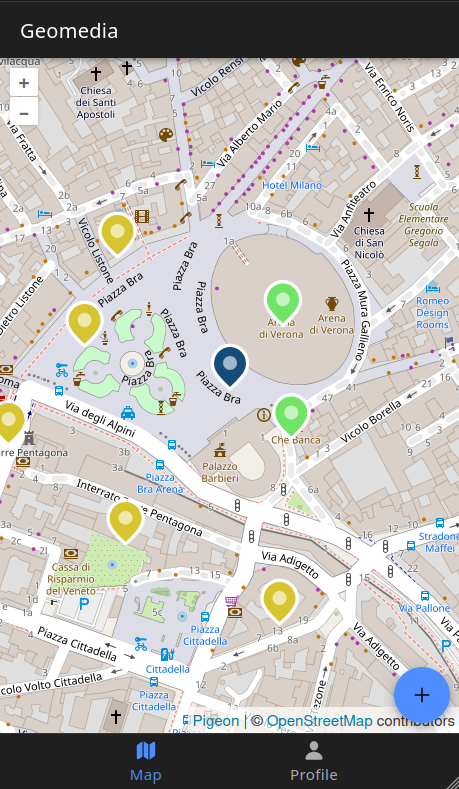
\includegraphics[width=4.8cm, height=9.5cm\textwidth]{imgs/Screenshots/CentroExclusive.png}}
\end{center}
\caption{Exclusive retrieving.}
\label{fig}
\end{figure}


This feature gives live to several use cases, for example GeoMedia could be used to create interactive experiences and games such as: ``scavenger hunt" or ``hide and seek" games.


\subsection{View post}

Another key component is the ``ViewPost" as represented in Figure 4, which shows the content in the clicked marker by opening a new interface and fetching the server to retrieve any associated multimedia data.
Media file attached in a post are retrieved only when the post is going to be opened and not at the start of the application (instead of the list of relative all location markers) due  to efficiency.
\\
This component is not limited to just viewing the comment; it also provides the functionality to download the attached multimedia file and store it in the local storage of the mobile device.
Media files are stored as ``Base64" encoding into the data-layer, so the client is also able to encode and decode the attachments.
\\
The owner of the comment, of course, is able to delete it.

\begin{figure}[htbp]
\begin{center}
\fbox{{\includegraphics[width=4.8cm, height=9.5cm\textwidth]{imgs/Screenshots/ViewPost.png}}}
\end{center}
\caption{Example of Post View.}
\label{fig}
\end{figure}


\subsection{HTTP requests}

The custom function doRequest() shown in the snippet of the Map component (Listing 1) is a wrapper to do an HTTP request to the server.
In fact, clients communicate with the server by adopting the HTTP protocol, then exchanging ``XHR" (XMLHttpRequest) packets whose contains data in JSON (JavaScript Object Notation) format encapsulated into the body of the POST method of HTTP.
\\
As follows, the code of doRequest method.
\begin{lstlisting}[language=Java, caption=Method doRequest to fetch server]
//various import 
import { Storage } from '@ionic/storage';
const store = new Storage(); 
store.create(); //start the cache storage
export const doRequest = (api, body = {}) => {
    return store.get("ServerConfig").then(ServerConfig => { //get config from cache
        return fetch("http://" + ServerConfig.ipserver + ":" + ServerConfig.port + "/" + api, {
            method: "POST",
            mode: "cors",
            body: JSON.stringify(body)
        }).then(res => res.json()).then(res => {
            return res;
        }).catch(err => {
            return err;
        });
    })
}
\end{lstlisting}


To simplify the server configuration in the app, has been installed the ``Ionic Storage" \cite{b9} packet, which allows to store data into the application's cache installed in the mobile phones. In order to use this feature an installation is required via terminal command: 
\begin{lstlisting}[language=Sh]
$ npm install @ionic/storage
\end{lstlisting}



\subsection{Ionic Capacitor}

To access physical sensors on Android, such as geolocation and file storage, Ionic Capacitor\cite{b10} can be integrated into the Ionic Framework project. Capacitor is a collection of libraries that make possible the use of native components inside web applications, then providing the API to adopt at JavaScript level.

Geomedia require two specific modules of Capacitor, in specific:
\begin{itemize}
    \item GeoLocation\cite{b2}: In way to get latitude and longitude coordinate of user logged into the app
    \item FileSystem\cite{b3}: In order to store file into mobile filesystem whenever users want to download the media uploaded
\end{itemize}

These plugins can be installed via a shell command, respectively:
\begin{lstlisting}[language=Sh]
$ npm install @capacitor/geolocation
$ npm install @capacitor/filesystem
\end{lstlisting}

The geolocation package provides the method getCurrentPosition() which returns an Object with properties: latitude, longitude, altitude; and for each attribute the accuracy.
\\
The altitude, even if not relevant for this project, could be integrated in future development thus to create more peculiar scenarios or use cases.


\subsection{Building for Android}

A key strength of the Ionic Framework is its ability to build web applications into native mobile apps; in fact, the framework acts as a wrapper/interpreter for the webpage, essentially embedding a custom browser inside the app.
\\
In order to create an Android Package (APK) for installing the app, some shell commands are required as reported in the official documentation, such as:
\begin{lstlisting}[language=Java]
`npm install @capacitor/android'  //to add the capacitor
$ npm install @capacitor/filesystem
`npx cap add android' //to denote the android platform, since IonicFramework can also build for "iOS" operating system
`npx cap build android' 
\end{lstlisting}
With the last command, the application will be deployed in production mode and then encapsulated into a bundle that later will be compiled by Android Studio \cite{b11} tool and the relative SDK.



At this point, the Android Manifest needs to be modified, by adding the opportune permissions which the users will grant when requested on startup/installation of the app.
\\
The only permission requested is the access to location, if denied the application will not work; a potential solution to avoid this scenario is to use the proximal location provided by antennas of the IPS, but could results in a very different position than the real one.

\\
Another customization is to allow clear traffic (HTTP), because since from Android 8 only HTTPS packets are allowed by default.
In fact, HTTP protocol is an insecure format where data is not encrypted and it's intended to be used just in the development phase, so the explicit declaration in the manifest is required in way to make the Android OS create an exception.

\begin{lstlisting}[language=XML, caption=Snippet of Android Manifest]
<application
    ...
    android:requestLegacyExternalStorage="true"
    android:largeHeap="true"
    android:usesCleartextTraffic="true"
>
...
</application>
...
<uses-permission android:name="android.permission.ACCESS_COARSE_LOCATION" />
<uses-permission android:name="android.permission.ACCESS_FINE_LOCATION" />
<uses-feature android:name="android.hardware.location.gps" />
        
\end{lstlisting}

\section{HTTP Server}

The HTTP server takes place as application layer, which represent the bridge between data stored and the client application explained before.
The GeoMedia HTTP server uses NodeJS\cite{b4} as engine to start a listening process on a designated network port; even more, the server exposes several paths called endpoints, each of which correspond to a specific function within the application. 
Each path handled by the server has a relative execution command of an SQL stored procedure, passing by parameters the input data and reading the result set as outcome to return to the client.
\\
The packages handled in this platform are in JSON (JavaScript Object Notation) content-type thus to allow a rapid extendability of data included and providing an easily human-readable format.
Only the ``POST" method is implemented, since every request/response include data and parameters encapsulated inside the body of the HTTP packet.
\\
The server requires just one external dependency not included natively, which is ``tedious"\cite{b5} (installable via `\$ npm install tedious') a module to establish a connection to Microsoft SQL Database (DBMS) then to execute query commands and transactions.

\begin{lstlisting}[language=Java, caption=Snippet of GeoMedia HTTP server]
const http = require("http");
const port = 9911
http.createServer((req, res) => {
    let body = "";
    req.on("data", (chunk) => {
        body += chunk
    });
    req.on("end", () => {
        ...
            body = JSON.parse(body)
        ...
        switch (req.url) {
            case "/doLogin": //LOGIN OR REGISTER
                dispatcher.doLogin(body.username, body.password, body.newuser).then(resQuery => {
                    sendResponse(res, 200, resQuery) //this method sends back the data
                }).catch(err => {
                    sendResponse(res, 500, err)
                })
                break;
            ....
           case "/getPosts":
                dispatcher.getPosts(body?.LATITUDE, body?.LONGITUDE,body?.USERNAME).then(resQuery=>{
                    sendResponse(res,200,resQuery)
                }).catch(err=>{
                    sendResponse(res,500,err)
                })
                break
            ...
            default:
                sendResponse(res, 404, { 'msg': "Unknown path:" + req.url })
                break;
        }
    })
}).listen(port);
\end{lstlisting}


The dispatcher class is just a helper, used to wrap the execution of SQL stored procedure and manipulate data whenever necessary.
\\
For example:
\begin{lstlisting}[language=Java, caption=snippet example of dispatcher.js class]
const SQL_MANAGER = require("./SQL_MANAGER"); //wrapper for tedious package 

function checkAREA(areaKM, post_latitude, post_longitude, curr_latitude, curr_longitude) {

    var dLat = (post_latitude - curr_latitude) * Math.PI / 180;
    var dLon = (post_longitude - curr_longitude) * Math.PI / 180;
    var a = 0.5 - Math.cos(dLat) / 2 + Math.cos(curr_latitude * Math.PI / 180) * Math.cos(post_latitude * Math.PI / 180) * (1 - Math.cos(dLon)) / 2;

    d = Math.round(6371000 * 2 * Math.asin(Math.sqrt(a))); // in meters
    if (d <= areaKM * 1000) { //transform areaKM to meters
        return true
    } else {
        return false
    }
}

async function getPosts(curr_latitude = null, curr_longitude = null, username = null) {
   
    let posts = await SQL_MANAGER.selectQuery(SQL_MANAGER.loadConfig(), "EXEC GETPOSTS @USERNAME='" + username + "'")

    let results = []
    posts.forEach(pp => {
        if (pp.AREA_KM != null) { // check if users' position is within the post availability
            if (checkAREA(pp.AREA_KM, pp.LATITUDE, pp.LONGITUDE, curr_latitude, curr_longitude)) {
                results.push(pp)
            }
        } else {
            results.push(pp)
        }
    })
    return results

}
function getMediaPost(postid){
    return SQL_MANAGER.selectQuery(SQL_MANAGER.loadConfig(),"EXEC GETMEDIAPOST @POSTID="+postid)
}

\end{lstlisting}


\subsection{Vincenty's formulae for distance computation}\label{server:screening}

As shown in Listing 5, the filtering for exclusive content is done partially in the application layer.
In fact, server executes the respective SQL stored procedure into the DBMS which already filters the expired posts limited by date, then server computes the visible radius of each exclusive post, then returns just the ones within the users' current location.

The method to compute the distance among the current user location requesting the posts and the position of the limited content within the kilometers chosen, is an implementation of Vincenty's formulae \cite{Vincenty}.
\\
This method was developed in 1975 by Thaddeus Vincenty \cite{ThaddeusVincenty} a Polish American geodesist who worked with the U.S. Air Force and later the National Geodetic Survey, and is based on the assumption that the Earth is an oblate spheroid, and hence are more accurate than methods that assume a spherical Earth, such as great-circle distance \cite{GCDWiki}. 

For GeoMedia application, has been implemented just the first method of Vincenty's solution, which computes the location of a point that is a given distance and azimuth (direction) from another point with an accuracy within 0.5 mm on the Earth ellipsoid.


\subsection{Microservices}
In the monolithic architecture designed, the server represents a single access node, which is a fragile solution in a real-world scenario, as it represents a ``single point of failure" where the failure of this node makes the whole system unavailable.
\\
There are many alternatives to mitigate this event. A potential approach is to replicate the HTTP server across different machines, introducing the challenge of synchronizing multiple main servers.
\\
A more sophisticated solution is to change the whole design, creating a distributed architecture by adopting microservices\cite{b6}. In this scenario, server is fragmented into multiple smaller processes that act one for each specific function, as theorically shown in Figure 5.
For example, one microservice could handle the post retrieval process, another could manage the accounts, another the creation of the posts, and so on. This approach not only improves reliability but also helps to distribute traffic loads thus to preventing the system from an overwhelmed; a common problem with social media platforms when a mass requests of a viral content happens, causing the ``break the Internet" \cite{BreakTheInternet} effect.


\begin{figure}[htbp]
\begin{left}
\fbox{{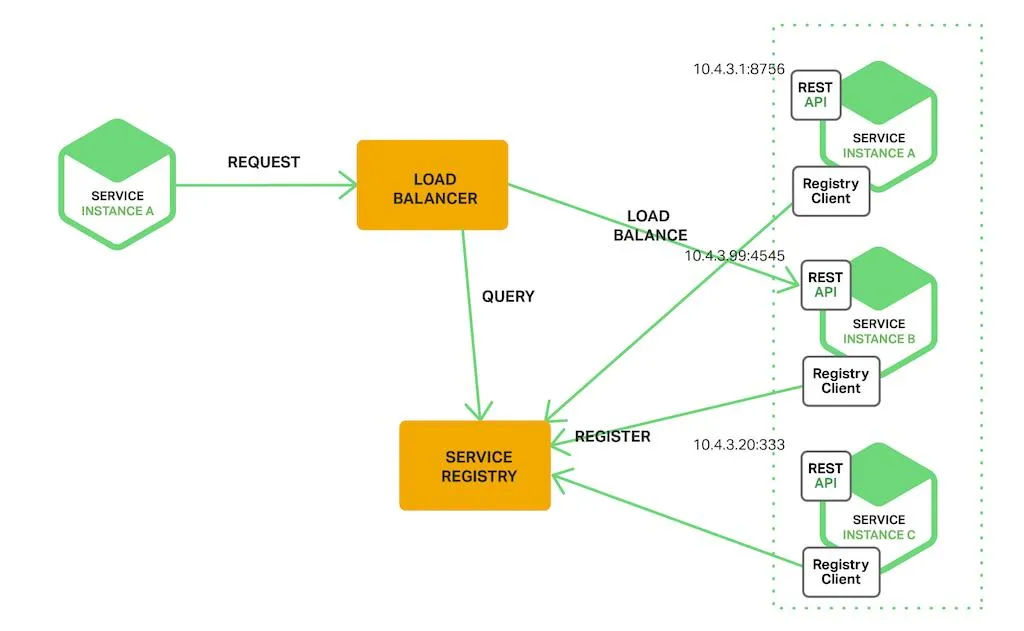
\includegraphics[width=8.5cm, height=5cm\textwidth]{imgs/microservices.png}}}
\end{lef}
\caption{Example of microservices architecture. \cite{b6}}
\label{fig}
\end{figure}



\section{DBMS}

Following the three-tier design, DBMS (DataBase Management System) represents the Data-layer, providing the function to maintain and to query data in it. Microsoft SQL Server (MSSQL)\cite{b7} has been selected to implement this role.
\\
All the posts and user profiles present in GeoMedia are stored in dedicated structure, specifically in database table:
\begin{itemize}
    \item `USERS' for users' profiles
    \item `POSTS' for posts 
\end{itemize}

\begin{lstlisting}[language=SQL, caption=Tables creation]
CREATE TABLE USERS(
    ID INT IDENTITY,
    USERNAME VARCHAR(50) PRIMARY KEY,
    PASSWORD NVARCHAR(256) NOT NULL, --stored the hash of MD5 function
);
CREATE TABLE POSTS(
	ID INT IDENTITY PRIMARY KEY,
	AUTHOR VARCHAR(50) FOREIGN KEY REFERENCES USERS(USERNAME),
	TITLE VARCHAR(50),
	COMMENT VARCHAR(MAX),
	MEDIATYPE VARCHAR(100), -- IMAGE/JPG, AUDIO/M4A
	MEDIADATA NVARCHAR(MAX), --BASE64
	POSTDATETIME DATETIME,
	COORD_X FLOAT,
	COORD_Y FLOAT,
);
\end{lstlisting}

Data is handled through stored procedures, which give to the data layer isolation and independency from the rest of architecture, so further modification (both to application or data layer) would not impact each other.
In example, when storing a post, all the the content and the author are passed as parameters, then manipulated and formatted into the opportune stored procedure inside the DBMS.

\begin{lstlisting}[language=SQL, caption=Stored Procedure of post creation]
CREATE PROCEDURE NEWPOST
@AUTHOR VARCHAR(50), @POSTCONTENT NVARCHAR(MAX)
AS
BEGIN
	INSERT INTO POSTS(AUTHOR,TITLE,COMMENT,MEDIATYPE,MEDIADATA,POSTDATETIME, LATITUDE, LONGITUDE)
	SELECT @AUTHOR, JJ.title, JJ.comment, JJ.mediatype, JJ.media_b64,GETDATE(), JJ.latitude ,JJ.longitude 
	FROM OPENJSON(@POSTCONTENT,'$') WITH(
		title  VARCHAR(50),
		comment  VARCHAR(MAX),
		media_b64  NVARCHAR(MAX),
		mediatype  VARCHAR(100),
		latitude FLOAT,
		longitude FLOAT
	) JJ
END;

\end{lstlisting}


\section{Future extensions}

In conclusion, GeoMedia offers a platform for sharing content on a geographic map. As previously mentioned, there are some key features that could be expanded.

TODO: richiama i related works

Some ideas include:

\subsection{Time capsule}

Extending the concept of limiting the content to a specific area, another idea could involve storing posts in small sensors distributed randomly in places such as forests, mountains, or cities. 
These sensors would be reachable only with short-range medium like Bluetooth or Wi-Fi, or even NFC.
\\
This idea gives life to several use cases, such as a waypoints to mark hiking routes in the mountains, or actings time capsules at panoramic points.


\begin{thebibliography}{00}
\bibitem{b1} Ionic Framework is cross-platform framework to create web-application and export them to mobile platform. http://www.overleaf.com
\bibitem{b2} Ionic Capacitor - Geolocation package to access to GPS location on mobile devices. https://capacitorjs.com/docs/apis/geolocation
\bibitem{b3}Ionic Capactor - FileSystem package to store data on mobile devices https://capacitorjs.com/docs/apis/filesystem
\bibitem{b4} NodeJS as server engine https://nodejs.org/en
\bibitem{b5}{Tedious - Node Package able to handle SQL Server communication}. https://tediousjs.github.io/tedious
\bibitem{b6} Microservices panoramic and image in figure https://medium.com/the-modern-scientist/introduction-to-microservices-architecture-f0c7efe79f1
\bibitem{b7} Microsoft SQL Server 2022 as DBMSQ for data layer https://www.microsoft.com/en-us/sql-server/sql-server-2022
\bibitem{b8} Pigeon Map as React Component to render a geographical map. https://pigeon-maps.js.org
\bibitem{b9}Ionic Storage to store the configuration of server. https://ionicframework.com/docs/react/storage
\bibitem{b10}Ionic Capacitor official website as documentation for the modules installed. https://capacitorjs.com
\bibitem{b11}Android Studio SDK official website, as a tool for building the Android APK. https://developer.android.com/studio
\bibitem{b12}React JS as chosen front-end framework. https://react.dev/
\bibitem{gh}GitHub public repository for GeoMedia project. https://github.com/albertomorini/GeoMedia
\bibitem{Vincenty} Vincenty solutions of geodesics on the ellipsoid. 
https://www.movable-type.co.uk/scripts/latlong-vincenty.html
\bibitem{ThaddeusVincenty} Bibliography of the Polish American geodesist Thaddeus Vincenty. https://en.wikipedia.org/wiki/Thaddeus\_Vincenty
\bibitem{GCDWiki}Great-circle distance or spherical distance method.
https://en.wikipedia.org/wiki/Great-circle\_distance
\bibitem{BreakTheInternet} Break the Internet effect. https://dictionary.cambridge.org/dictionary/english/break-the-internet
\bibitem{GoogleMaps} Google Maps as social media, provided by Google. https://en.wikipedia.org/wiki/Google\_Maps
\bibitem{StreetView} Street View, functionality of Google Maps.
https://en.wikipedia.org/wiki/Google_Street_View
\bibitem{Instagram} Instagram, Online Social Media owned by Meta Platforms, Inc.
\bibitem{Meta} Meta Platforms, Inc.
https://en.wikipedia.org/wiki/Meta_Platforms
\bibitem{Instagram Stories} Instagram stories functionality, to publish time-limited content
https://about.instagram.com/features/stories
\bibitem{MetaPrivacy}Meta Accused Of Still Flouting Privacy Rules With AI Training Data
https://www.forbes.com/sites/emmawoollacott/2025/05/15/meta-accused-of-still-flouting-privacy-rules-with-ai-training-data/
\bibitem{FourSquareWiki} Foursquare City Guide as City explorer social media.
https://en.wikipedia.org/wiki/Foursquare\_City\_Guide
\bibitem{FoursquareOfficialLink} Foursquare's official home page.
https://foursquare.com/
\bibitem{FoursquareSwarm} Foursquare's SwarmApp official home page.
https://www.swarmapp.com/
\end{thebibliography}

\vspace{12pt}

\end{document}
